%%=============================================================================
%% Methodologie
%%=============================================================================

\chapter{\IfLanguageName{dutch}{Methodologie}{Methodology}}%
\label{ch:methodologie}

%% TODO: In dit hoofstuk geef je een korte toelichting over hoe je te werk bent
%% gegaan. Verdeel je onderzoek in grote fasen, en licht in elke fase toe wat
%% de doelstelling was, welke deliverables daar uit gekomen zijn, en welke
%% onderzoeksmethoden je daarbij toegepast hebt. Verantwoord waarom je
%% op deze manier te werk gegaan bent.
%%
%% Voorbeelden van zulke fasen zijn: literatuurstudie, opstellen van een
%% requirements-analyse, opstellen long-list (bij vergelijkende studie),
%% selectie van geschikte tools (bij vergelijkende studie, "short-list"),
%% opzetten testopstelling/PoC, uitvoeren testen en verzamelen
%% van resultaten, analyse van resultaten, ...
%%
%% !!!!! LET OP !!!!!
%%
%% Het is uitdrukkelijk NIET de bedoeling dat je het grootste deel van de corpus
%% van je bachelorproef in dit hoofstuk verwerkt! Dit hoofdstuk is eerder een
%% kort overzicht van je plan van aanpak.
%%
%% Maak voor elke fase (behalve het literatuuronderzoek) een NIEUW HOOFDSTUK aan
%% en geef het een gepaste titel.

This section contains a brief description of the road map to build the proof of concept (PoC), which combines the general key insights from the literature. Within the methodology a brief description is provided about each experiment, without specifying actual results or code implementations. These can be found in \ref{ch:results}

The proposed model can be seen as a three-way modular setup, jumper localization, action segmentation and skill recognition.
Each step can be improved individually in order to acquire the best possible result and is implemented independently.
The first step focuses on localizing the athletes in the field in order to crop them out and spare computational resources. Next up is segmenting each skill performed in a given routine. The final part involves recognizing each isolated skill.

All experiments are performed using an Acer Nitro ANV15-51, running Ubuntu 24.04.2 LTS, using a 13th Gen Intel® Core™ i5-13420H × 12, with 16GB RAM and a NVIDIA GeForce RTX™ 4050 Laptop GPU 5898MiB.

% TODO : chart overview of model.

\section{Genral information}

Before jumping into each different step, some general information is provided. Each of the 458 DD3 freestyles collected, 2231 total videos, has a record in the database. Two selections have been made to decide the videos in the validation set. The first selection is filtering all videos of this season (67 videos). The second selection uses the id of the video. In the beginning of the project, taking the 10th modulo of the id being 5 resulted in the most validation videos. Currently this corresponds to 42 validation videos. The other 90\% are used as training videos (349).
Each recording lasts for about 60 to 75 seconds, depending on the competition level and has around 40 to 60 performed skills. These do not include normal jumps. In order to annotate the videos, a custom Vue3 web application is created. In order to render the videos in the browsers, conversions from blu-ray (m2ts) or AVI to mp4 were required. Most videos have a framerate of 25, 30 or 50 frames per second (fps), while some may be 15, 28 or 60.
The quality of videos differ and range from anywhere between 8 and 550MB. It may not indicate much, but just to keep in mind. Even on the more qualitative videos, the rope disappears when making quick rotations. This is often better on higher fps videos.

\section{Jumper localization}
\label{methodology:jumper-localization}

Jumper localization is needed in order crop a zoomed-in video of the skippers performing their routine. Image \ref{fig:sr4-field} perfectly illustrates a competition setting, where the majority of the video is lost on surroundings, judges and spectators. The field is typically 12 by 12 meters for the athletes to use.

\begin{figure}
    \centering
    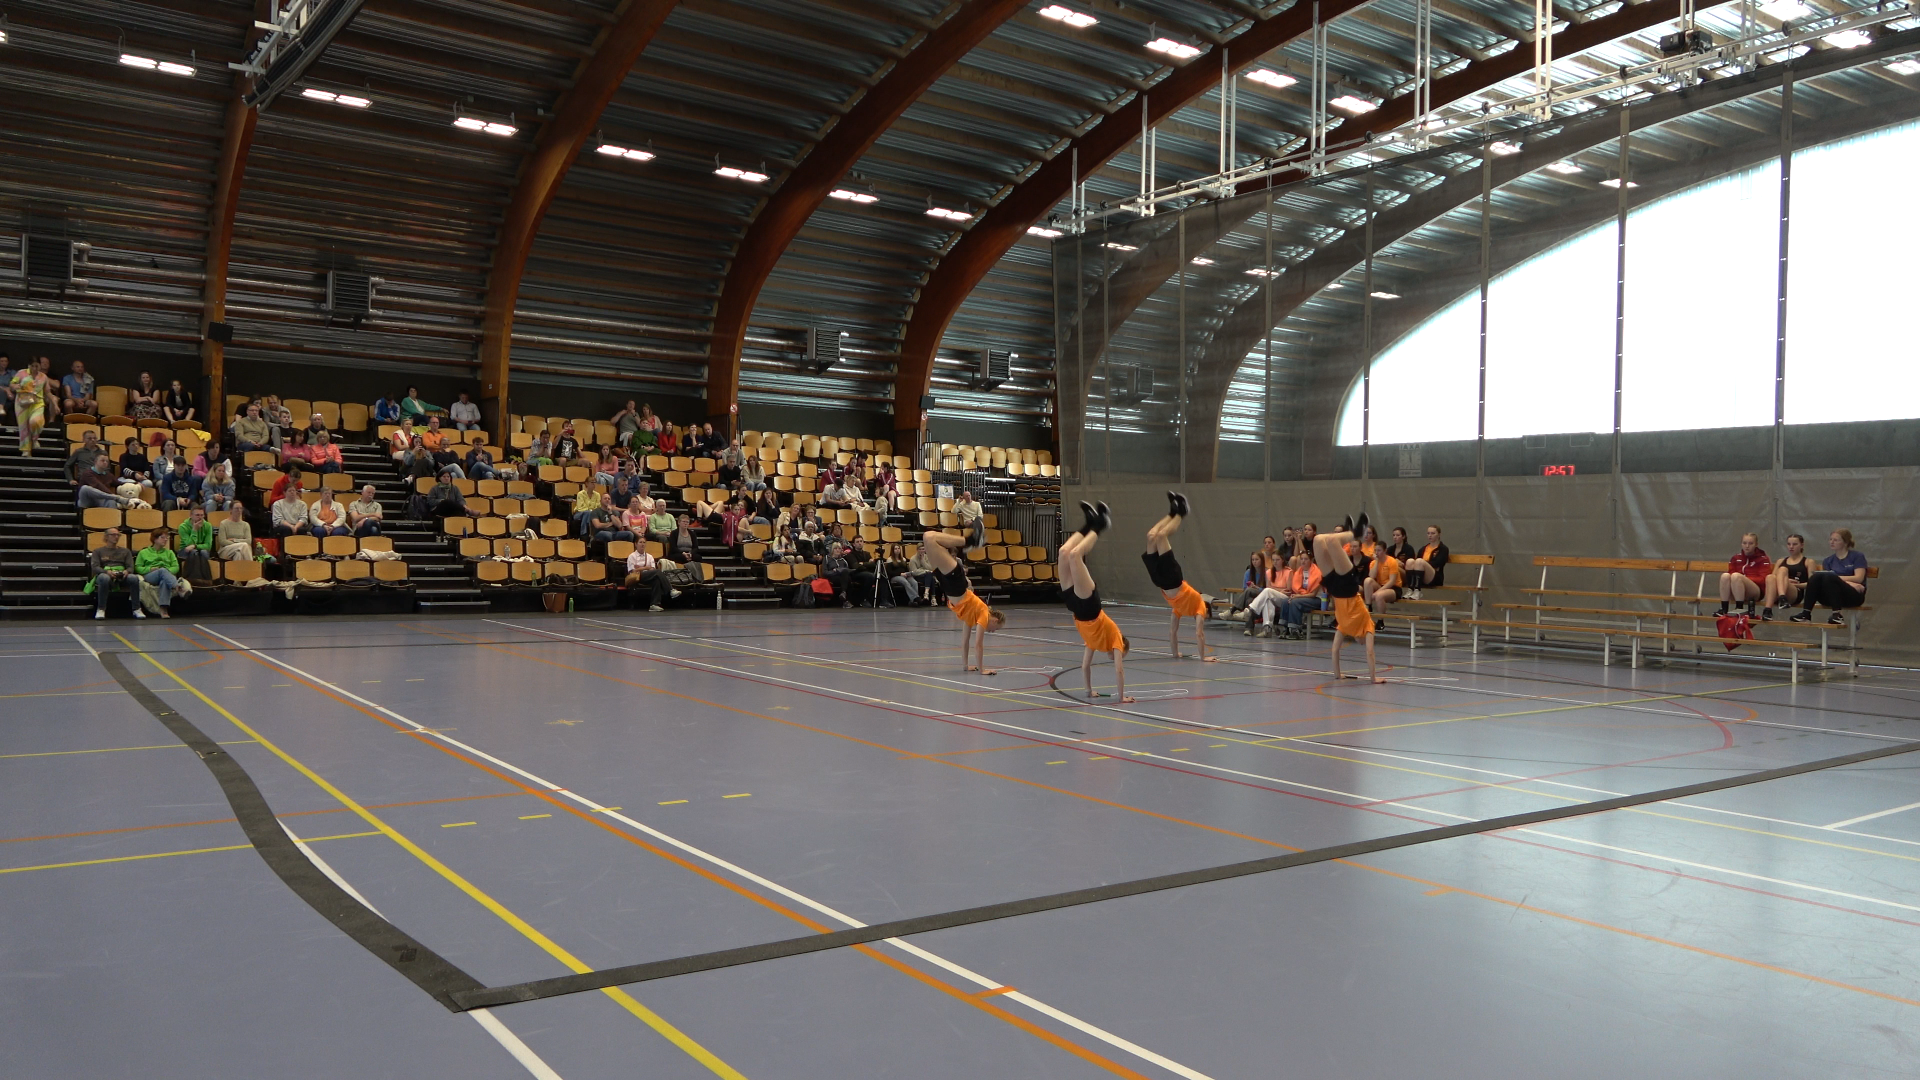
\includegraphics[width=0.95\linewidth]{sr4-field}
    \caption[Example jump rope competition setting]{Example of a competition setting in which four athletes are performing a SR4 freestyle.}
    \label{fig:sr4-field}
\end{figure}

Experiments on localizing implement two major ways of labeling athlete locations, full team boxes and individual boxes.
For this project the relative center point along the x-axis, y-axis, width and height of the box are stored. So regardless of the scale of the image, whether the image has size 1920 x 1080 pixels or 1080 x 720 pixels, the position of the box remains the same.
This way, by scaling all images to the same size, frames of dimension (width, height, channels) can fed into the model, giving 4 values in return. An example of a box would be [0.6, 0.5, 0.4, 0.4], all values range between 0 and 1.
Team labels require one box for a single image, contrary to multiple boxes for individual athletes.
After training and predicting box coordinates, the Jaccard similarity coefficient otherwise known as the Intersection over Union accuracy (IoU) can be performed evaluating the performance of the model. This allows for comparison of models or training rounds.

Full team predictions were experimented on MobileNetV3 \autocite{Howard2019} and GoogleNet \autocite{Szegedy2014}. Labeling some frames of almost any DD3 routine, variety in the leftover data was limited. This marked the transition towards individual labels.

% TODO Vision Transformer?
Ultralytics, \autocite{Khanam2024}, provides an easy way to implement their YOLO models. For this research, YOLOv11 is used to predict individual boxes, providing satisfying results \ref{results:yolo}.
Using the predicted locations of the skippers, each frame of video can be cropped around the athletes. Results weren't perfect, sometimes visual disturbing, because of sudden zoom outs, blurry athletes or predictions of spectators. This required smoothing techniques to improve full video crops \ref{results:crop-stability}.

Manually reviewing full cropped videos is time consuming, requiring automated tests in order to check full video crops. The implementation of these automated tests used the full team boxes comparing the minimum IoU overlaps for each video, as these moments mattered most. By manually checking videos, problematic moments were additionally labeled as full team boxes. However, the further development and full video crop results were unfinished and put on hold due to time constraints.

\section{Action segmentation}
\label{methodology:action-segmentation}

The main purpose of the action segmentation is to enable predictions on full routines in order to actually use the whole model. Using the cropped images, and the assigned start and end frame of a skill, the model can predict whether a given frame is an interesting split point or not.

For jump rope, this mostly means moments when an athlete leaves or lands on the floor. However there are special cases such as cartwheels. Only moments when either hands or feet land over a rope, are annotated as the end of a skill.
To annotate which moments are interesting split points, the start and end frame of a skill receive value 1, while other frames remain 0.
As the start and end frame of a skill are rather subjective, frames around a split point also range somewhere between 0 and 1. These values are calculated using the function \ref{code:calculate-splitpoint-values} which is called on in the data generator demonstrated in code \ref{code:call-splitpoint-calculation}.
Each frame than has a value from zero to one. An example of consecutive splitpointvalues could be:

\([0, 0, 0.1, 0.31, 0.55, 0.86, 1, 0.86, 0.55, 0.31, 0.1, 0]\)

Having a splitpoint value for each frame of the video, the video can be partioned into consecutive sections of T timesteps. Because the Multiscale Vision Transformer is pre-trained on videosections of 16 frames, the same amount of timesteps are taken to finetune the model for segmentation. This makes the model transform the input of size (batch size, channels, timesteps, height, width) into an output of size (batch size, timesteps).

Available experiments include code implementations of the Video Vision Transformer (ViViT) as introduced in \textcite{Arnab2021} and the Self-Attention ConvLSTM from \textcite{Lin_2020}. Both models showed the same results, averaging out predictions slightly above 0 for all frames, stagnating on MSE losses, not actually grasping what happens in given sections of frames it receives.

The final experiment on action segmentation uses \href{https://pytorch.org/vision/main/models/video_mvit.html}{PyTorch's Video MViT}, which is an implementation based on the Multiscale Vision Transformer created by \textcite{Fan2021} which can be finetuned using the pre-trained weights on the kinetics dataset \autocite{Kay2017}. This experiment will be elaborated in section \ref{results:action-segmentation-mvit}.


\section{Skill recognition}
\label{methodology:skill-recognition}

The last part involves recognizing each performed skill, which is, as introduced in the literature, a combination of different aspects. What are the turners doing, using one or both arms, an additional body rotation, etc.
For this part, a video vision model is definitely required to fill in the temporal information, e.g. amount of rotations.

One minor issue, is about skills differing in duration. One might take half a second, the other might be 800 milliseconds.
This can be solved by ensuring they have the same length of T = 16 timesteps, skipping or duplicating frames. This resulted in equal sized inputs with dimensions (channels, timesteps, height, width) or (C, T, H, W) for short.

Next up was transforming all aspects of skills into machine understandable output labels. This was the reason why the skill matrix has been created \ref{lit:skill-matrix}. The matrix resulted in a skill configuration \ref{code:confighelper} for skill labels, specifying 13 different outputs; Type, Rotations, Turner1, Turner2, Skill, Hands, Feet, Turntable, BodyRotations, Backwards, Sloppy, Hard2see and Fault. Each aspect being a category, numeric value or a boolean.

Along the way, additional aspects to a skill label can be added in order to incorporate for every level and skill variation.
Furthermore, once-in-a-lifetime skills can be marked as unknown in order for the model to be robust in predicting new skills. After analyzing the given skillsection, a level can be assigned, based on the predicted aspects.
Multiple different models can be tested in order to find the best one.

The first experiments implement the Video Vision Transformer and the Self-Attention ConvLSTM, which averaged out the most occurring aspects; normal jumps, no mistakes, 1 rotation...
These models were trained on upsampeled data, increasing occurrences of more unique skill combinations.

Following unsuccessful trials trained from scratch, accelerated the implementation of the Multiscale Vision Transformer for recognizing skills. At the same time, in order to test things out, skills where limited to to a balanced 5 class dataset; jumps, return from powers, pushups, frogs and other skills, hoping for better results.
The results where excellent, even starting to recognize aspects of turners, quickly re-enabling predictions on all skills \ref{results:mvit}.

Further experiments added other models, namely video ResNet models or Swin Transformers \ref{results:skill-recognition-resnet-swin-saconv3d} or adjusted the returned losses, based on skill aspect occurrence in the dataset during training and validation \ref{results:skill-recognition-weighted-loss}.

\section{Judge score comparison}
\label{methodology:judge-score-comparison}

Finally, when skills are predictable, a comparison between the jury assigned scores, the models prediction and the effective score can be made in order to check whether model predictions could be used or more research/training is needed. This is an important check, verifying usability on competitions \ref{results:skill-recognition-act-as-a-judge}.

